\documentclass[12pt,a4paper,utf8]{ctexart}
\usepackage{graphicx}
\usepackage{amsmath}
\usepackage{amssymb}
\usepackage{subfig}
\usepackage{cite}
\usepackage[ntheorem]{empheq}
\usepackage{enumitem}
\usepackage{fullpage}
\usepackage{cleveref}
\usepackage{cellspace}
\usepackage{listings}
\usepackage{color}
\usepackage{float}
\definecolor{gray}{rgb}{0.5,0.5,0.5}
\definecolor{dkgreen}{rgb}{.068,.578,.068}
\definecolor{dkpurple}{rgb}{.320,.064,.680}

% set Matlab styles
\lstset{
   language=Matlab,
   keywords={break,case,catch,continue,else,elseif,end,for,function,
      global,if,otherwise,persistent,return,switch,try,while},
   basicstyle=\ttfamily,
   keywordstyle=\color{blue}\bfseries,
   commentstyle=\color{dkgreen},
   stringstyle=\color{dkpurple},
   backgroundcolor=\color{white},
   tabsize=4,
   showspaces=false,
   breaklines,%自动换行
   showstringspaces=false,
   numbers=left,   % 行号的位置在左边
   columns=fixed,
}

\begin{document}
\CJKfamily{zhkai}


\begin{center}
   \textbf{作业三}\\
   \textbf{敖旭扬 ~~~~~ PB18071477 ~~~~~ \today}\\
\end{center}
\textit{}
\vspace{\baselineskip}

\begin{enumerate}
   \item[第一题] 解:
   \item[\textbf{(a)}]
         由Gauss顺序消元法的步骤和过程,第一次迭代后$A$的第一列完成消去时,有
         \begin{eqnarray}
            \begin{aligned}
               a_{ij}^{(1)}=a_{ij}-\dfrac{a_{i1}}{a_{11}}a_{1j},\quad i,j=2,3,\cdots,n
            \end{aligned}
         \end{eqnarray}
         由于$A$是对称矩阵且满足$a_{11} \neq 0$,所以有
         \begin{eqnarray}
            \begin{aligned}
               a_{ij}=a_{ji},\quad i,j=1,2,3,\cdots,n
            \end{aligned}
         \end{eqnarray}
         所以
         \begin{eqnarray}
            \begin{aligned}
               a_{ij}^{(1)}=a_{ij}-\dfrac{a_{i1}}{a_{11}}a_{1j}=a_{ji}-\dfrac{a_{1i}}{a_{11}}a_{j1}=a_{ji}-\dfrac{a_{j1}}{a_{11}}a_{1i}=a_{ji}^{(1)},\quad i,j=2,3,\cdots,n
            \end{aligned}
         \end{eqnarray}
         从而$A^{(1)}$是对称的。
   \item[\textbf{(b)}]
         计算一个正定(positive definite)矩阵LU分解的算法如下:
         \lstinputlisting[frame=single]{src/LU.m}
   \item[\textbf{(c)}]
         使用Cholesky分解解方程组$Ax = b$的\textsc{Matlab}程序显示如下:
         \lstinputlisting[frame=single]{src/p1c.m}

         根据上述程序在命令行输出的结果(以注释形式写在了上面的代码中),
         原题所求的解为:
         \begin{eqnarray}
            \begin{aligned}
               x=\begin{bmatrix}
                  1 \\
                  2 \\
                  1 \\
                  2
               \end{bmatrix}
               \nonumber
            \end{aligned}
         \end{eqnarray}

   \item[第二题] 解:
   \item[\textbf{(a)}] 证明:\\
         Richardson迭代方法的迭代关系式为:
         \begin{eqnarray}
            x^{(k+1)}=\omega I(\frac{1}{\omega}I-A)x^{(k)}+\omega Ib=(I-\omega A)x^{(k)}+\omega b
         \end{eqnarray}
         令
         \begin{eqnarray}
            G_\omega =I-\omega A
         \end{eqnarray}
         则
         \begin{eqnarray}
            x^{(k+1)}=G_\omega x^{(k)}+\omega b
         \end{eqnarray}
         根据课本第五章开头处对迭代法收敛性的讨论可知,上述Richardson 迭代方法收敛的充要条件为
         谱半径$\rho(G_\omega)<1$,又$A$是正定矩阵,所以它的特征值均为正数,由已知,$G_\omega$的特征值为$1-\omega \lambda_i$,其中
         $0<\lambda_1 \leq \lambda_i \leq \lambda_n$,则
         \begin{eqnarray}
            \rho(G_\omega)=max|1 − \omega \lambda_i|<1
         \end{eqnarray}
         则对任意$\lambda_i$,需要满足
         \begin{eqnarray}
            0<\omega \lambda_i<2
         \end{eqnarray}
         即
         \begin{eqnarray}
            \omega<2/\lambda_n
         \end{eqnarray}
   \item[\textbf{(b)}]
         由\textbf{(a)}得,
         \begin{eqnarray}
            \rho(G_\omega)=\max|1 − \omega \lambda_i| = \max(1 − \omega \lambda_1,\omega \lambda_n-1)
         \end{eqnarray}
         应该使得收敛速度尽量快,所以$\rho(G_\omega)$应该尽量小,即取
         \begin{eqnarray}
            \rho(G_\omega)=\min_\omega \max(1 − \omega \lambda_1,\omega \lambda_n-1)
         \end{eqnarray}
         所以$\omega$的最佳值为
         \begin{eqnarray}
            \omega_b = \arg \min_\omega \max(1 − \omega \lambda_1,\omega \lambda_n-1)=\dfrac{2}{\lambda_1+\lambda_n}
         \end{eqnarray}
         且
         \begin{eqnarray}
            \rho(G_\omega)=\left\{
               \begin{array}{rcl}
               1 − \omega \lambda_1 & & {\omega \leq \omega_b}\\
               \dfrac{\lambda_n-\lambda_1}{\lambda_n+\lambda_1} & & {\omega = \omega_b}\\
               \omega \lambda_n-1 & & {\omega \geq \omega_b}
               \end{array} \right.
         \end{eqnarray}
   \item[\textbf{(c)}] 
         使用Richardson迭代方法解$Ax = b$的\textsc{Matlab}程序显示如下:
         \lstinputlisting[frame=single]{src/p2c.m}
         上述程序某一次执行输出的结果为:
         \lstinputlisting[frame=single,numbers=none]{src/p2c_outs.txt}
         同时输出的收敛迭代次数随$\omega$变化的semilogy图为:
         \begin{figure}[H]
            \centering
            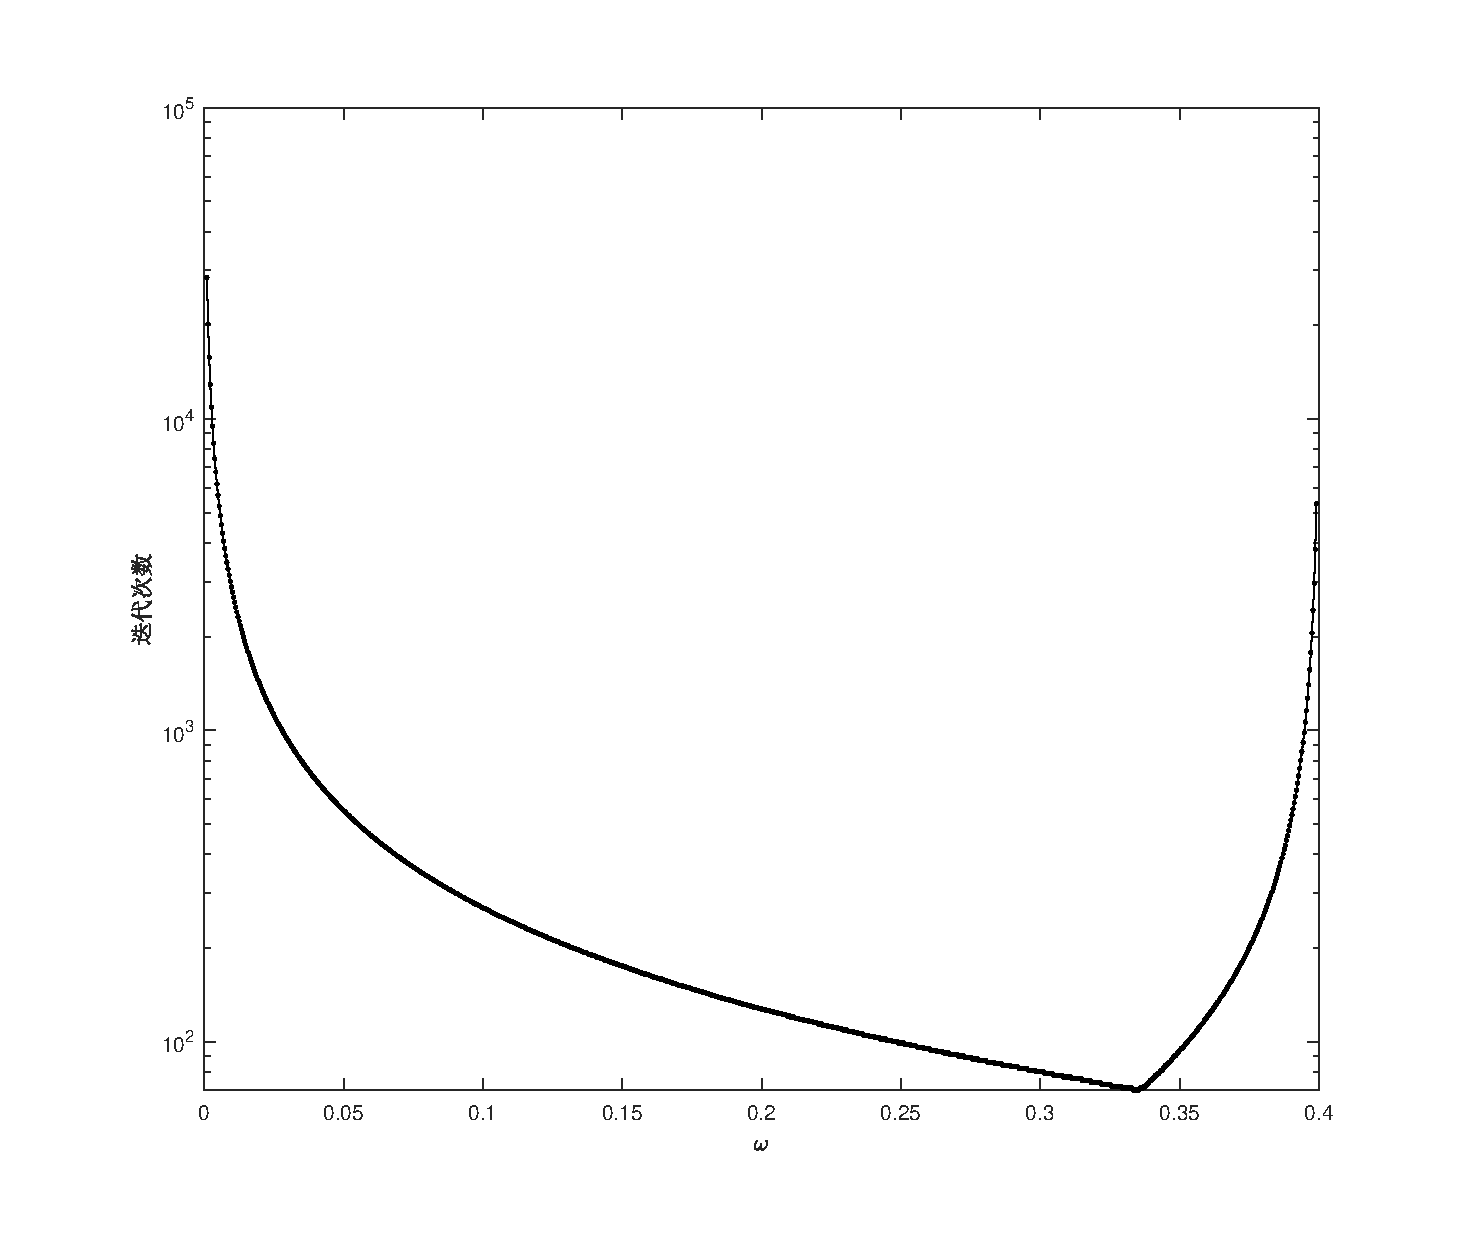
\includegraphics[width=1\textwidth]{fig/p2c.eps}
            \caption{寻找Richardson迭代方法的最佳$\omega$}
         \end{figure}
         这一结果验证了最佳$\omega$是$\omega_b$,它使得收敛速度最快。
   \item[第三题] 解:
   \item[\textbf{(a)}]$I(f)=\int_a^b f(x) \mathrm{d} x$关于积分节点$\{x_1,x_2,\cdots,x_n\}$的Gauß积分的数值积分公式为
   \begin{eqnarray}
      I_n(f)=\sum_{i=1}^n\alpha_if(x_i)
   \end{eqnarray}
   $n=6$时,代数精度不超过$2n-1=11$,所以依次取线性不相关的$f(x)=1,x^2,\cdots,x^{10}$,即$f_k(x)=x^{2k},\quad k=0,1,\cdots,5$,根据
   \begin{eqnarray}
      I_n(f)=I(f)
   \end{eqnarray}
   取$a=-1,b=1$得
   \begin{eqnarray}
      \sum_{i=1}^6\alpha_{i} x_i^{2k} =\int_{-1}^{1} x^{2k} \mathrm{d}x=\dfrac{2}{2k+1} \quad,\quad k=0,1,\cdots,5 \label{equp3a1}
   \end{eqnarray}
   又根据Gauß的节点和积分权重关于原点对称,即
   \begin{eqnarray}
      \alpha_{i}=\alpha_{i+3},\quad x_i=-x_{i+3},\quad i=1,2,3 \label{equp3a3}
   \end{eqnarray}
   所以式$(\ref{equp3a1})$变为
   \begin{eqnarray}
      \sum_{i=1}^6\alpha_{i} x_i^{2k} = 2\sum_{i=1}^{3}\alpha_{i} x_i^{2k} =\dfrac{2}{2k+1} \quad,\quad k=0,1,\cdots,5
   \end{eqnarray}
   即
   \begin{eqnarray}
      \sum_{i=1}^{3}\alpha_{i} x_i^{2k} =\dfrac{1}{2k+1} \quad,\quad k=0,1,\cdots,5
   \end{eqnarray}
   写成方程组则表示为
   \begin{eqnarray}
      \begin{cases}
             \sum\limits_{i=1}^{3}\alpha_{i} =1
         \cr \sum\limits_{i=1}^{3}\alpha_{i} x_i^{2} =\dfrac{1}{3}
         \cr \sum\limits_{i=1}^{3}\alpha_{i} x_i^{4} =\dfrac{1}{5}
         \cr \sum\limits_{i=1}^{3}\alpha_{i} x_i^{6} =\dfrac{1}{7}
         \cr \sum\limits_{i=1}^{3}\alpha_{i} x_i^{8} =\dfrac{1}{9}
         \cr \sum\limits_{i=1}^{3}\alpha_{i} x_i^{10} =\dfrac{1}{11}
         \end{cases} \label{equp3a2}
   \end{eqnarray}
   \item[\textbf{(b)}]方程组$(\ref{equp3a2})$中一共有$\langle \alpha_1,\alpha_2,\alpha_3,x_1,x_2,x_3\rangle$共$6$个变量,
   且有
   \begin{eqnarray}
      \begin{aligned}
      \dfrac{\partial \Big(\sum\limits_{i=1}^{3}\alpha_{i} x_i^{2k}\Big)}{\partial \alpha_j}&=x_j^{2k}\\
      \dfrac{\partial \Big(\sum\limits_{i=1}^{3}\alpha_{i} x_i^{2k}\Big)}{\partial x_j}&=2k\alpha_jx_j^{2k-1}\quad(k\neq 0)\\
      \dfrac{\partial \Big(\sum\limits_{i=1}^{3}\alpha_{i}\Big)}{\partial x_j}&=0
      \end{aligned}
      \nonumber
   \end{eqnarray}
   其中$j=1,2,3;\quad k=0,1,2,3,4,5$\\
   所以非线性方程组$(\ref{equp3a2})$的Jacobian的表达式为
   \begin{eqnarray}
      \begin{aligned}
         \boldsymbol{J}&=\dfrac{\partial \Big(\sum\limits_{i=1}^{3}\alpha_{i},\sum\limits_{i=1}^{3}\alpha_{i} x_i^{2},
         \sum\limits_{i=1}^{3}\alpha_{i} x_i^{4},\sum\limits_{i=1}^{3}\alpha_{i} x_i^{6},
         \sum\limits_{i=1}^{3}\alpha_{i} x_i^{8},\sum\limits_{i=1}^{3}\alpha_{i} x_i^{10}\Big)}{
            \partial(\alpha_1,\alpha_2,\alpha_3,x_1,x_2,x_3)
         }\\
         &=\begin{bmatrix}
            1 & 1 & 1 & 0 & 0 & 0  \\
            x_1^2 & x_2^2 & x_3^2 & 2\alpha_1 x_1 & 2\alpha_2 x_2 & 2\alpha_3 x_3  \\
            x_1^4 & x_2^4 & x_3^4 & 4\alpha_1 x_1^3 & 4\alpha_2 x_2^3 & 4\alpha_3 x_3^3  \\
            x_1^6 & x_2^6 & x_3^6 & 6\alpha_1 x_1^5 & 6\alpha_2 x_2^5 & 6\alpha_3 x_3^5  \\
            x_1^8 & x_2^8 & x_3^8 & 8\alpha_1 x_1^7 & 8\alpha_2 x_2^7 & 8\alpha_3 x_3^7 \\
            x_1^{10} & x_2^{10} & x_3^{10} & 10\alpha_1 x_1^9 & 10\alpha_2 x_2^9 & 10\alpha_3 x_3^9 
         \end{bmatrix}
      \end{aligned}
   \end{eqnarray}
   \item[\textbf{(c)}] 求解$n = 6$情况下的Gauß积分的积分节点和积分权重的\textsc{Matlab}程序显示如下:
      \lstinputlisting[frame=single]{src/p3c.m}
      上述程序在命令行的输出结果为
      \lstinputlisting[frame=single,numbers=none]{src/p3c_out.txt}
      所以积分节点和积分权重为
      \begin{eqnarray}
         \begin{aligned}
        (x_1,x_2,x_3)&=(-0.932469514203152,-0.661209386466265,-0.238619186083197)\\
        (\alpha_1,\alpha_2,\alpha_3)&=(0.171324492379170,0.360761573048139,0.467913934572691)
        \nonumber
         \end{aligned}
      \end{eqnarray}
      其中其他几项由式$(\ref{equp3a3})$得到。\\
      这里初始权重的选取是根据课本(第三版)第130页下方的$\alpha_i^{(n)}$公式计算而来(但是把其中的$x_i^{(n)}$用$x$初始值代替了)。
   \item[\textbf{(d)}]\textsc{Matlab}程序显示如下:
   \lstinputlisting[frame=single]{src/p3d.m}
\end{enumerate}

\end{document}
